\documentclass{article}
\usepackage{graphicx}
\usepackage[margin=1 in]{geometry}

\title{Lip Reading with Multimodal Speech Recognition}
\author{Abhinav Reddy | Ankita Agarwal | Arjun Surendran \\ Nazim Shaikh | Suchismita Sahu}
\date{}
\begin{document}
\maketitle


\section{INTRODUCTION}
In Real World, lipreading is the skill of recognizing what is being said from visual information. It is a challenging problem because of the ambiguity at the word and phoneme level that visual information contains. Multiple sounds share the same shape. For example visemes - different phonemes that produce the same lip sequence  (e .g 'ah' and 'aa', 'p' and 'b').\cite{LipreadingInWild} Visual lipreading plays an important role in human-computer interaction in noisy environments where audio speech recognition is difficult. It can also be extremely useful as a means of communication for the hearing-impaired. In addition, there can be several potential applications like dictating messages in noisy environment and better dealing with multiple simultaneous speakers.In recent years, Machine Learning has been more effective than professional lip readers in discerning speeches from the silent video clips.\cite{MultimodalMlReview}

The idea behind this project is to make use of visual information of the stance of the mouth or lip region in addition to the corresponding audio to predict spoken phonemes\cite{MultimodalAVSR}. Our work is inspired from the state of the art lipreading algorithm called LIPNET\cite{LIPNET}, developed by researchers at the University of Oxford which makes use of spatiotemporal convolutions, a recurrent network, and the connectionist temporal classification(CTC)loss, trained entirely end-to-end to give sentence-level lipreading.

We implement a similar multimodal system\cite{gpm12} which makes use of video as well as audio features to improve the performance of the lipreading system on a phoneme level. The video sub\-network is trained on a sequence of images passing through several layers of CNN-LSTM \cite{LipreadingCNN} for extracting temporal information\cite{garg2016lip} and the audio sub\-network has LSTM layers with attention mechanism \cite{Attention_Medium} both ultimately retrieving the final sequence of phoneme sequence spoken.

\section{LITERATURE REVIEW}
In this section, we outline various existing approaches to automated lipreading.
\subsection{Automated Lipreading}
 Most existing work on lipreading does not employ deep learning. Such work requires either heavy preprocessing of frames to extract image features, temporal pre-processing of frames to extract video features (e.g., optical flow or movement detection), or other types of handcrafted vision pipelines (Matthews et al., 2002; Zhao et al., 2009; Gurban \& Thiran, 2009; Papandreou et al., 2007; 2009; Pitsikalis et al., 2006; Lucey \& Sridharan, 2006; Papandreou et al., 2009). Generalization across speakers and extraction of motion features is considered an open problem, as noted in a recent review article (Zhou et al., 2014). LipNet\cite{LIPNET} addresses both of these issues.
\subsection{Classification with Deep Learning}
In recent years, there have been several attempts to apply deep learning to lipreading. However, all of these approaches perform only word or phoneme classification, whereas LipNet\cite{LIPNET} performs full sentence sequence-to-sequence prediction. Approaches include learning multimodal audio-visual representations (Ngiam et al., 2011), learning visual features as part of a traditional speech-style processing pipeline (e.g. HMMs, GMM-HMMs, etc.) for classifying words and/or phonemes (Almajai et al., 2016; Takashima et al., 2016; Noda et al., 2014; Koller et al., 2015), or combinations thereof (Takashima et al., 2016). Many of these approaches mirror early progress in applying neural networks for acoustic processing in speech recognition (Hinton et al., 2012). Chung \& Zisserman (2016a) propose spatial and spatiotemporal convolutional neural networks, based on VGG, for word classification. The architectures are evaluated on a word-level dataset BBC TV (333 and 500 classes), but, as reported, their spatiotemporal models fall short of the spatial architectures by an average of around 14\%. Additionally, models cannot handle variable sequence lengths and they do not attempt sentence-level sequence prediction. 
Chung \& Zisserman (2016b) train an audio-visual max-margin matching model for learning pre\-trained mouth features, which they use as inputs to an LSTM for 10-phrase classification on the OuluVS2 dataset, as well as a non-lipreading task. Wand et al. (2016) introduce LSTM recurrent neural networks for lipreading but address neither sentence-level sequence prediction nor speaker independence. This work holds the previous state-of-the-art in the GRID corpus with a speaker-dependent accuracy of 79.6\%. Garg et al. (2016)\cite{garg2016lip} apply a VGG pre-trained on faces to classifying words and phrases from the MIRACL-VC1 dataset, which has only 10 words and 10 phrases. However, their best recurrent model is trained by freezing the VGGNet parameters and then training the RNN, rather than training them jointly. Their best model achieves only 56.0\% word classification accuracy, and 44.5\% phrase classification accuracy, despite both of these being 10-class classification tasks.

\subsection{Sequence prediction in speech recognition}
The field of automatic speech recognition (ASR) would not be in the state it is today without modern advances in deep learning, many of which have occurred in the context of ASR (Graves et al., 2006; Dahl et al., 2012; Hinton et al., 2012). The connectionist temporal classification loss (CTC) of Graves et al. (2006) drove the movement from deep learning as a component of ASR, to deep ASR systems trained end-to-end (Graves \& Jaitly, 2014; Maas et al., 2015; Amodei et al., 2015). As mentioned earlier, much recent lipreading progress has mirrored early progress in ASR, but stopping short of sequence prediction. No lipreading work (based on deep learning or not) has performed sentence-level sequence prediction. LipNet demonstrates the first sentence-level results by using CTC. Furthermore, it does not require alignments to do so.


\section{DATASET AND PREPROCESSING}
The dataset used in this audio-visual SR is the TCD-TIMIT dataset created by Trinity College, Dublin which has 13826 video clips in MP4 format of 59 Volunteers and 3 Lipspeakers reading a total of 6913 phonetically rich sentences and labeled phoneme-wise. There are other well known datasets such as GRID and VidTIMIT. However, we didn't choose them because either they had short repetitive sentences or had low video quality. We choose to use the reduced 39 phoneme set in accordance to Lee and Hon et.al and choose 3 lipspeakers who each speak 377 sentences and 1 Volunteer sub\-part from the entire dataset because of better state-of-the art accuracy and performance is obtained for lipspeakers. 

\subsection{AUDIO PREPROCESSING}
\subsubsection{Resampling}
The audio data in the dataset is sampled at 48kHz. We downsample the audio data at 16kHz to reduce computational complexity of processing the data and to make comparison of performance easier and considering the fact that high sampling rate is not useful for speech recognition. 
\subsubsection{MFCC Extraction}
The Mel-Frequency Cepstral Coefficients are extracted with a window frame of 25ms with 10ms overlap using Librosa library. We used 13-dimensional MFCC features and the phoneme labels corresponding to each MFCC frame are generated from the labelfiles included in the dataset.
The MFCC features are stacked with overlapping in an array to be further fed to the Neural Network. Eg 1-9 2-10 (Timesteps is 9) And the label for each row is the label of the central frame. 


\subsection{VIDEO PREPROCESSING}
The TCD-TIMIT videos were recorded at straight face angle with a large area focused around the speakers head. However for our task, only the region around the mouth is of relevance\cite{Mouthshapes}. The phoneme labelfiles are used to find out the timestamps that correspond to a spoken phoneme. It is assumed that the phoneme is most clearly visible on the mouth exactly between the start and end timestamp; the timestamp of the middle of this interval is then converted to the frame number in the video. After knowing the video frame numbers of all phonemes, \cite{Thesis}
\begin{enumerate}
\item The relevant frames are extracted using a python script that makes use of ffmpeg\cite{CNNFeatures}
\item The face of the speaker as well as mouth is detected using Dlib\cite{Dlib}
\item The face and mouth are converted to grayscale images to reduce the size of the data and hence the training time
\item The mouth images are resampled to 120$\times$120 pixels [50] to provide a constant input size to the CNN
\item The image pixel values are then normalized to [0,2] and centered around zero so that results are in the interval [-1,1] to improve performance
\end{enumerate}

\section{NETWORK ARCHITECTURE}
\subsection{AUDIO SUBNETWORK}
\subsubsection{LSTM}
Long Short-Term Memory Networks (LSTM) \cite{LipreadingLSTM} are a special kind of Recurrent Neural Networks, capable of learning long-term dependencies. An issue with standard feed-forward networks is that they can't take into account time information. This is however extremely important for speech recognition. When a person has pronounced ’c’ and ’a’, the next letter might very well be an ’r’. The probability of it being ’t’ is quite low. LSTMs\cite{LSTM} can use this time information by adding a kind of memory to the network in the form of internal states via gates.
Here, A 2 layer LSTM network with 256 units/layer is implemented in the audio network and single layer LSTM network with 256 units/layer is deployed in the video network.
\begin{figure}
\centering
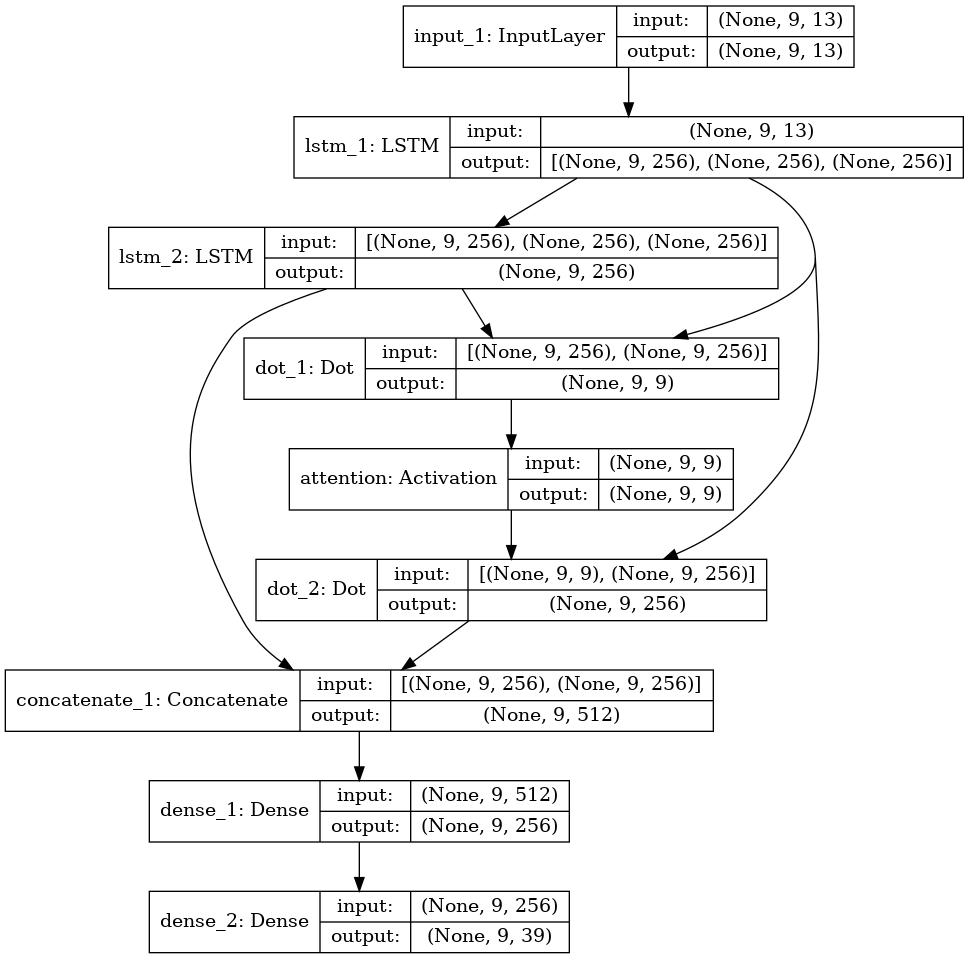
\includegraphics[scale=0.4]{audio_model_plot.png}
\caption{\label{fig:Audio SubNetwork Architecture}The Audio Subnetwork with Attention Mechanism}
\end{figure}

\subsubsection{ATTENTION NETWORK}
Attention Mechanisms in Neural Networks are (very) loosely based on the visual attention mechanism found in humans. \cite{Attention_memory} The Attention Encoder-Decoder architecture is popular because it has demonstrated state-of-the-art results across a range of domains.\cite{Attention_ML} From a high-level, the model is comprised of two sub-models: an encoder and a decoder.
\begin{enumerate}
    \item Encoder: The encoder is responsible for stepping through the input time steps and encoding the entire sequence into a fixed length vector called a context vector.
    \item Decoder: The decoder is responsible for stepping through the output time steps while reading from the context vector.
\end{enumerate}
Key to the model is that the entire model, including encoder and decoder, is trained end-to-end, as opposed to training the elements separately. Attention is proposed as a solution to the limitation of the Encoder-Decoder model encoding the input sequence to one fixed length vector from which to decode each output time step. This issue is believed to be more of a problem when decoding long sequences. Instead of decoding the input sequence into a single fixed context vector, the attention model develops a context vector that is filtered specifically for each output time step. This is achieved by keeping the intermediate outputs from the encoder LSTM layer from each step of the input sequence and training the model to learn to pay selective attention to these inputs and relate them to items in the output sequence in decoder LSTM layer. Putting in another way, each item in the output sequence is conditional on selective items in the input sequence.


\subsection{VIDEO SUBNETWORK}
\subsubsection{CNN}
With the extensive use of image processing involved in lip reading task, Convolutional Neural Networks (CNNs) are the best networks to be used here\cite{Imagenet}. They are quite similar to normal FCNNs, but are organized in a different way. Neurons connect only to a small part of the neurons from the previous layer, not to all of them. This reduces the number of network parameters enormously. CNNs are always multi-layered.
A CNN generally follows the structure shown below. It consists of convolutional (CONV) layers, nonlinearity layers (NonLin), pooling layers (POOL), and fully connected layers (FC).
\newline
\newline
Input $\rightarrow$ [CONV $\rightarrow$ NonLin $\rightarrow$ POOL] *N $\rightarrow$ [FC]*M $\rightarrow$ FC(softmax)
\newline
\newline
A summary of the important properties of a CNN:
\begin{enumerate}
\item CONV layers convolve a number of filters across the height and width of the volume of neurons in the previous layer.
\item POOL layers to reduce the size of the data by downsampling along width and height. There are different types of pooling - Max Pooling, Average Pooling, and L2-Norm Pooling.
\item FC layers at the end perform classification
\end{enumerate}
We explored several CNN architectures such as CIFAR10, GoogleNet(Inception), VGGNet, Resnet50. The CNN network used for lip reading in the paper \cite{LipreadingInWild} was found to work quite well experimentally compared to others and was therefore used in this work with slight modification. The WLAS network offers a good compromise between performance, complexity and speed of training as it has limited number of CONV output features but not too few, so there is not much loss of information when these features are used in further network layers. It consists of five CONV layers with ReLu activations and four POOL layers performing max-pooling. Additionally, we introduced batch normalization\cite{BatchNormalization} layer after each of the first three Max-POOL layers to get a better parameter-to-data ratio. 
\begin{figure}
\centering
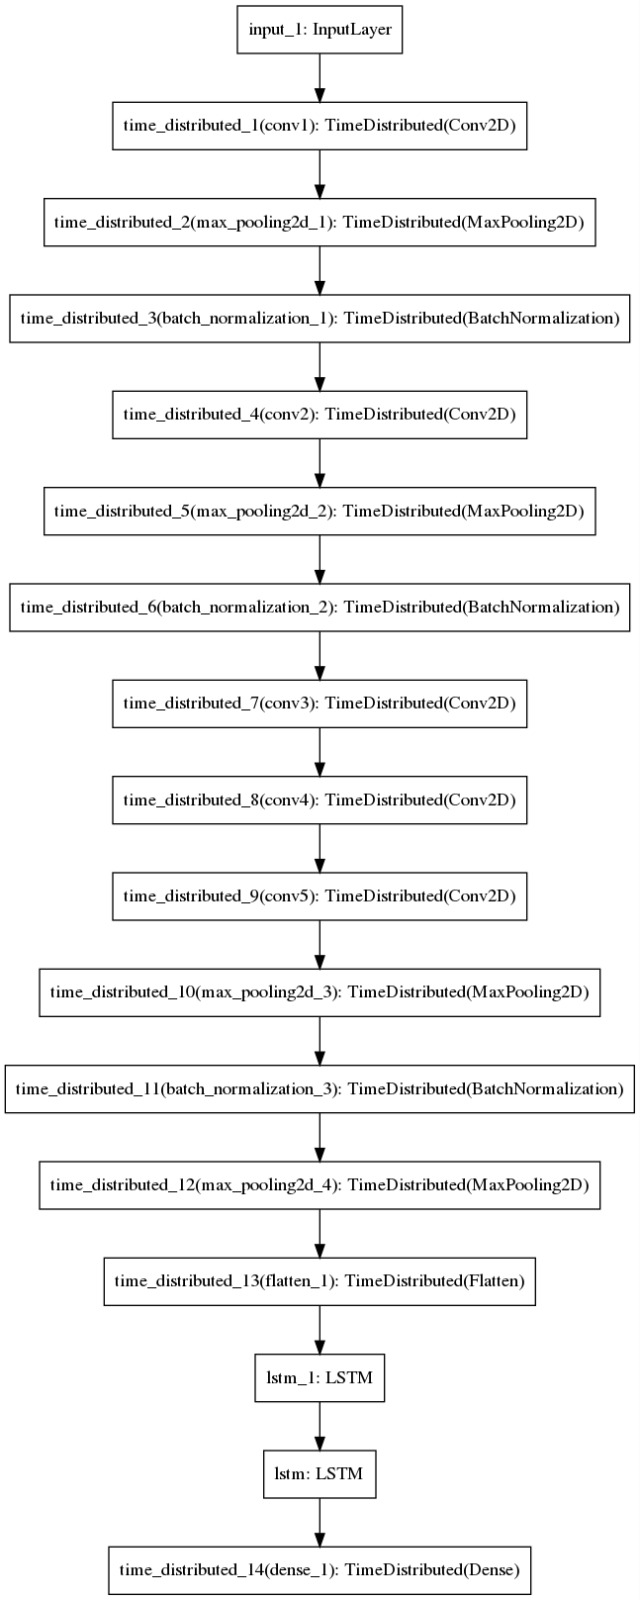
\includegraphics[scale=0.52]{VideoModelPlot.png}
\caption{\label{fig:Video SubNetwork Architecture}The Video Subnetwork}
\end{figure}
\subsubsection{CNN\--LSTM}
In practicality, lipreading system will not be based on single images but on a sequence of images (a video), so it is ideal to use temporal information in conjunction with spatial information of images. This is done with the help of LSTMs. The LSTMs in audio subnetwork used the MFCCs of the processed audio data as inputs, which contained a sequence of timeframes, with several features per timeframe. Similarly, the image frames from a video can be converted to a sequence of features that a LSTM can use as inputs: a CNN processes each of the images sequentially, and the output features are stored in a sequence that the LSTM can use.\cite{blendingLSTMCNN}
\subsubsection{FULLY CONNECTED LAYERS}
CNN-LSTM don't produce predictions of the classification labels, but selected features that were observed in the data. We use fully connected layer at the end makes use of these features to perform phoneme classification. 
\subsection{COMBINED NETWORK}
\begin{itemize}
    \item The predictions of the audio and video sub-networks are combined. 
    \item A single hidden layer fully connected network with 256 neurons is used for phoneme prediction from the combined predictions.
    \item The purpose of this network is to make a weighted prediction from outputs of both networks. In other words, it learns which of the two networks predicts certain phonemes better, and assigns weights accordingly.
\end{itemize}


\section{ARCHITECTURAL DETAILS}
\subsection{AUDIO SUBNETWORK}
The audio subnetwork takes in a sequence of MFCC features from each timeframe. The 'LSTM' blocks represent the LSTM network at different timesteps i.e timestamps when a phoneme is spoken in a video. The LSTM processes the input sequence one frame at a time. 
Now the attention mechanism\cite{Speech_Attention} generates an output sequence (phonemes) at each time step and selects or weighs the signals produced by LSTM at all of the time steps in the input sequence (speech frames). This weighted feature vector then helps to condition the generation of the next element of the output sequence.\cite{Attention_LSTM}.
\newline
Details of audio-attention sub-network:
\begin{enumerate}
    \item 2 layer LSTM with 256 units per layer one acting as encoder and the other acting as decoder\cite{Attention_Medium} which works along with the attention network\cite{Attention_ML}. The output of this is passed on to a Multi-Layer perceptron.
    \item MLP has 2 layers of Dense one with 256 neurons with tanh activation and next with 39 neurons with softmax activation to predict the probability of the phoneme sequence
\end{enumerate}.


\subsection{VIDEO SUBNETWORK}
The video subnetwork takes in a sequence of images which is passed through CNN blocks giving out selected features. The LSTM network processes the sequence formed by the outputs of CNN for all of the images. When combining CNN and LSTM networks in one architecture, some issues arise. The CNNs images output is a flattened 2D array but LSTM layers require a 3D input shape: (batchSizeLSTM, nbTimeFrames, numFeatures) to accomodate the extra timing information. Thus, we use TimeDistributed layers at CNN to take care of the extra time dimension. \cite{LAS}.
The frames extracted from a video sequence are processed in small batches within a CNN, while an LSTM runs on the CNN output sequentially in a time distributed manner to generate output characters. Dynamically, a N-frame sequence is grouped together in a block (width $\times$ height $\times$ N), where N is the number of frames in a single video. The N-sequence length is varying and the consecutive nature of the frames creates a spatiotemporal CNN.\cite{LIPNET} Then, the output of the LSTM layer is processed by Fully Connected Dense layers at each timestep to generate phoneme predictions for each image frame of the sequence.\cite{speechDecoding}

The input data is structured in the following arrays:
\begin{enumerate}
    \item X : contains the images as a numpy array with shape (nFrames, width, height, channels) i.e (38,120,120,1) where 38 here corresponds to number of frames in a single video. Pixel values are float32 numbers.
    \item y: contains the true labels of the images. The values are strings as the phonemes which are later label encoded and one hot encoded before passing to the network. 
\end{enumerate}

\subsection{COMBINED AUDIO-VIDEO SUBNETWORK}
We implement a modified version of the WLAS Network keeping only the Watch and Listen Layers and adding an FC layer for the combination. \cite{LipreadingInWild}
\begin{enumerate}
    \item Watch : (Image Encoder CNN-LSTM) Takes images in a sequence and encodes them into a deep representation to be processed by the network ahead. It looks at each frame in the video and extracts relevant features that the module has learned to look for i.e lip movements/positions.
    \item Listen : (Audio Encoder LSTM) Takes the 13-Dimensional MFCC features of the audio data as input. The LSTM generates a state vector(or cell state) and an output signal. The output is a phoneme prediction, while state is what encodes "the past", i,e what an LSTM has computed/stored of the past which is used to predict the next output.
    \item To combine the output of both the network, the number of frames i.e the frame-rate is required to be equal for audio and video. So, to make them consistent, we first find the difference in number of test labels between audio and video and then we up-sample the video predictions by that amount. Now, reshaped video predictions are combined with audio predictions and passed through a fully connected neural network to retrieve final video phoneme predictions.
\end{enumerate}
  
\section{TRAINING}
For the purpose of training, we chose lipspeaker dataset. The reason is that being professional lipspeakers, their mouth movements are more distinct and therefore the phonemes and corresponding visemes would be easier to learn because of the prominent mouth features.
Both audio and video subnetworks were trained separately for 30 epochs and performance was observed. When performance didn't improve after a patience of 5-10 epochs, training was stopped using early stopping and the best model was saved.
\newline
Both subnetworks were trained with below configurations:
\newline
\newline
Audio Subnetwork:\newline
Total trainable Network parameters \cite{LSTMParams}: 943,143 \newline
Loss Metric : Categorical Cross-entropy \newline
Optimizer : Adam \newline
\newline
Video subnetwork:\newline
Total Trainable Parameters:\cite{CNNFeatures} 19,173,351 \newline
Loss Metric : Categorical-cross-entropy \newline
Optimizer : Adam \newline
\newline
The Combined network was trained using fixed subnetworks meaning that lipreading and audio networks were trained seperately and the best trained models were saved and loaded. So, during training of the combined network, only the weights of the FC combination layers was trained.
Mean squared error was used loss functions along with Adam optimizer for learning rate optimization.

\section{COMPLEXITY ANALYSIS} 
The audio network and CNN are chosen to maintain a good balance between complexity and performance and is the same for all trained multimodal networks. CNNs require lots of computations. For CNN-based classifiers, over 90\% of the runtime is spent in the convolutional layers. Therefore most of the variation in complexity comes from the type of connections between the subnetwork. Weights in the CNN can be reused many times per image, and there\’s one image for each timeframe. Audio LSTM weights is used once per audio frame, of which there are more than one timeframes. Weights in the FC combining layers are used only once per time frame.  
Approximate training time was 5 mins per epoch for audio-network and 10-12 mins per epoch for video network. The combined network training took approximately 30 mins for 10 epochs.

\section{EXISTING CODEBASE}
The reference thesis \cite{Thesis} had existing work on the multimodalSR Lip Reading in Lasagne and Theano. We took reference from the same to preprocess our video data, extract frames and subsequently mouth regions from the frames, and map the timestamps to the label phonemes to create phoneme text files for the video data. For the audio data, we referred the code base to extract phoneme from the wav audio files. Apart from this, we used the code script to download the audio and video files from the TCD-TIMIT dataset with our own modifications for data restructuring.

\section{MAJOR CHALLENGES AND ADAPTATIONS}
\begin{enumerate}
    \item A lot of the phonemes are not visually distinguishable. Thus, the same viseme gets mapped to various phonemes. This means that when we map the visemes to phonemes we get the same image input for different phonemes resulting in a considerably low accuracy in the combined network.
    \item Building a network that performs well on our video data was a big challenge. We tried implementing different architectures for the CNN module in CNN-LSTM combination network. The model that best balances the weights and computational complexity was finally chosen.
    \item Synchronizing the audio-video data to get the combined prediction was challenging. Attention Network was implemented to combine the audio and video sub-networks and take care of the synchronization between the audio-video data but it did not give best results on our training data. So, we chose to combine the predictions of the two sub-networks into a final prediction of phonemes using a FC layer. 
    \item For improving the performance of video sub-network, we tried data augmentation on images but did not see improvement in results. We suspect that the results did not improve because the test data did not contain the image features that were used by the data augmentation. Implementing data augmentation made our system more robust but did not improve the classification accuracy. 
\end{enumerate}


\section{INDIVIDUAL CONTRIBUTIONS}
\begin{enumerate}
    \item Abhinav Reddy: Video Preprocessing, Data generator for network input, testing video model on standard CNN networks .
    \item Ankita Agarwal: Audio Preprocessing, Data Restructuring
    \item Arjun Surendran: Audio Preprocessing, Building and training audio subnetwork with attention, Combining audio-video subnetworks.
    \item Nazim Shaikh: Building and training video subnetwork, combining audio-video subnetworks.
    \item Suchismita Sahu: Literature review, Building video subnetwork, tuning and testing on various state of the art networks.
\end{enumerate}


\section{PERFORMANCE EVALUATION}
The trained network was first evaluated on the small test set of TCDTIMIT Lipspeakers. The test set is constructed in such a way that no speaker will have videos in both training and test set. This is done to evaluate the generalization capability of the model, i.e to make sure that the model is not speaker dependent. For performance measurement classification tasks, top-1 accuracy is used as a metric. For each input sample, the prediction of the network with the highest probability score is compared with the real label. If the prediction is correct, the evaluation is counted as correct. Otherwise, counted as wrong. The final top-1 accuracy score is then the fraction of samples that were predicted correctly compared to the total number of input samples.
The network is also evaluated on part of volunteer dataset of TCDTIMIT. Performance is significantly lower than for the lipspeakers. This is mainly due to speaker dependency of the trained networks, but also due to the fact that the lipspeakers' mouth movements are more distinct and easier to classify because the mouth features are more prominent.

\bigskip
\begin{tabular}{ |p{2cm}|p{2cm}||p{3cm}|p{3cm}|p{3cm}|  }
 \hline
 \multicolumn{5}{|c|}{TOP-1 ACCURACY} \\
 \hline
 Train Set & Test Set & Audio Subnetwork & Video Subnetwork & Audio-Video Combined Subnetwork \\
 \hline
 Lipspeaker & Lipspeaker & 70.51 & 37.5 & 41.12\\
 Lipspeaker & Volunteer & 53.2 & 25.67 & 31.95\\
 \hline
\end{tabular}
\bigskip

\section{CONCLUSION AND FUTURE WORK}
\begin{figure}
\centering
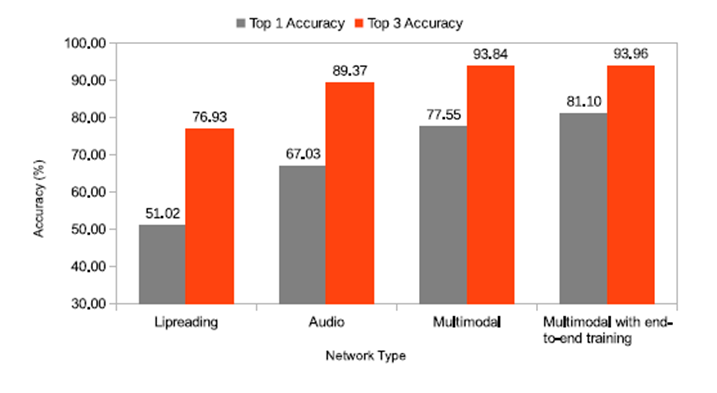
\includegraphics[scale=0.7]{SOTA.png}
\caption{\label{fig:Reference Results} Reference State of the Art Performance of the Audio, Video and Combined Multimodal Subnetworks}
\end{figure}
Multimodal lip reading is a challenging task mainly because of the similarity in the phonemes among various mouth shapes. To understand this we did audio only, video only and Combined audio-video network evaluation as tabulated. To further evaluate our model, we compare our results with that of reference thesis\cite{Thesis}. We see that multimodal network depends strongly on performance of audio network since audio-only recognition is considerably better than video-only classification performance. This is due to the fact that our model takes into consideration all the MFCC values for single phoneme keeping in mind the real world scenarios. As for the video sub-network and the combined Audio-Video sub-network, there's a lot more work left to do to improve the accuracy to a desirable level.
\newline \newline \newline
Proposed future work and improvements :
\begin{enumerate}
    \item Only a limited number of CNN types were explored and it could well be that other networks or variations on these networks perform better.
    \item Determining what factors exactly influence the performance could limit the accuracy loss and help improve accuracy.
    \item Adding a visual attention mechanism for lipreading as a way to save computation can further improve performance.
    \item Using the straight cam and the 30 degree video data instead of only straightcam to train the video sub-network might help improve accuracy.
    \item Training the networks with added noise might help the network be more robust,in turn improving the accuracy.
    \item Higher performance and better speaker-independence can be achieved if the networks are trained on larger and more varied datasets, e.g. diverse set of speakers of different nationalities.
    \item To make the speech recognition network more useful in practice it would be interesting to add a language model on top of the phoneme prediction network.
    \item To train the network on word or sentence-level predictions from the start, i.e end-to-end training for sequence to sequence\cite{sq2sq} prediction might give a better performance and training of the network, instead of training the audio and video sub-networks independently and freezing the respective best trained weights. We also intended to implement CTC: connectionist temporal classification loss as used in LipNet \cite{LIPNET} which may help improve the accuracy of the sequence prediction. 
\end{enumerate}

\bibliographystyle{plain}
\bibliography{bibliography.bib}
\end{document}

